\chapter{ऐल्कीन और ऐल्काइन: इलेक्ट्रॉनरागी योगज}\label{ch:b1:electrophilic-additions}

किसी ऐल्कीन को नारंगी ब्रोमीन जल के साथ हिलाइए, तो रंग कुछ ही सेकंड में
लुप्त हो जाता है: कार्बन--कार्बन द्वि-आबंध का सबसे पुराना परीक्षण। इसके पीछे एक
क्रियाविधि है। द्वि-आबंध के $\pi$ इलेक्ट्रॉन, जो
$\sigma$ इलेक्ट्रॉनों की तुलना में कम दृढ़ता से बँधे होते हैं और अणु के तल के ऊपर और नीचे खुले रहते हैं,
किसी इलेक्ट्रॉन-न्यून अभिकर्मक पर आक्रमण करते हैं; बना हुआ धनायन फिर
किसी \omterm{def:b1:electronic-effects:nucleophile}{नाभिकरागी} को ग्रहण करता है। यही दो चरण ऐल्कीनों पर हाइड्रोजन हैलाइड, जल
और हैलोजन जोड़ते हैं, तय करते हैं कि कौन-सा कार्बन अभिकर्मक का कौन-सा भाग
पाता है, और उत्पाद का त्रिविम रसायन निर्धारित करते हैं। यह अध्याय
उन्हें विकसित करता है, उस नियम के साथ जो उन्नीसवीं शताब्दी के एक रसायनज्ञ ने
प्रेक्षण से निकाला था, और उस \omterm{def:b1:electronic-effects:intermediates}{कार्बधनायन} के साथ जो उसकी व्याख्या करता है।

\begin{recall}
\omterm{def:b1:electronic-effects:intermediates}{कार्बधनायन}, उनका स्थायित्व और \omterm{def:b1:electronic-effects:curly-arrow}{वक्र तीर} (\cref{ch:b1:electronic-effects});
हैमंड अभिगृहीत (\cref{prop:b1:elementary-steps:hammond}); $Z$/$E$
वर्णक, \cip{R}/\cip{S}, \omterm{def:b1:stereochemistry-in-depth:enantiomers}{मेसो यौगिक} और \omterm{def:b1:stereochemistry-in-depth:enantiomers}{रेसेमिक मिश्रण}
(\cref{ch:b1:stereochemistry-in-depth})। विद्यालय के खंड (कक्षा 12) ने
ऐल्कीनों के योगों को उनकी क्रियाविधियों के बिना सूचीबद्ध किया था।
\end{recall}

\section{नाभिकरागी के रूप में \texorpdfstring{$\pi$}{पाई} आबंध}

\begin{definition}[इलेक्ट्रॉनरागी योगज]\label{def:b1:electrophilic-additions:electrophilic-addition}
किसी बहु-आबंध पर \emph{इलेक्ट्रॉनरागी योगज}\index{इलेक्ट्रॉनरागी योगज}
ऐसा योग है जिसका पहला चरण
$\pi$ इलेक्ट्रॉनों का किसी \omterm{def:b1:electronic-effects:nucleophile}{इलेक्ट्रॉनरागी} E पर आक्रमण है: एक धनायन बनता है, जो फिर
किसी \omterm{def:b1:electronic-effects:nucleophile}{नाभिकरागी} Nu को ग्रहण करता है, ताकि E और Nu पूर्व द्वि-आबंध के दोनों कार्बनों पर
पहुँच जाएँ।
\end{definition}

$\pi$ आबंध C=C के दोनों आबंधों में दुर्बलतर है (\cref{ch:b1:lewis-resonance-vsepr}),
और उसके इलेक्ट्रॉन नाभिकों से दूर, तल के ऊपर और नीचे, रहते हैं:
ऐल्कीन \omterm{def:b1:electronic-effects:nucleophile}{नाभिकरागी} हैं, और अम्लों, हैलोजनों और ऐसे अन्य
\omterm{def:b1:electronic-effects:nucleophile}{इलेक्ट्रॉनरागियों} से अभिक्रिया करती हैं जो संतृप्त ऐल्केनों को अछूता छोड़ देते हैं।

\section{हाइड्रोजन हैलाइडों का योग: मार्कोवनिकोव का नियम}

\begin{omfigure}
\setchemfig{atom sep=2.1em}
\schemestart
\chemfig{H_3C-[:30]@{c2}CH=[@{pi},,,,]@{c1}CH_2}
\+
\chemfig{@{h}H-[@{hb}]@{br}Br}
\arrow{->}
\chemfig{H_3C-[:30]CH^{+}-[:-30]CH_3}
\+
\chemfig{Br^{-}}
\arrow{->}
\chemfig{H_3C-[:30]CH(-[2]Br)-[:-30]CH_3}
\schemestop
\chemmove{\draw[->, thick, shorten <=2pt, shorten >=2pt](pi) .. controls +(90:7mm) and +(110:7mm) .. (h);
          \draw[->, thick, shorten <=2pt, shorten >=2pt](hb) .. controls +(-90:5mm) and +(-90:5mm) .. (br);}

{\small प्रोपीन पर हाइड्रोजन ब्रोमाइड का योग। $\pi$ युग्म
प्रोटॉन को अंतस्थ कार्बन पर ले लेता है, जिससे द्वितीयक \omterm{def:b1:electronic-effects:intermediates}{कार्बधनायन} बनता है;
ब्रोमाइड आयन उससे जुड़ता है: 2-ब्रोमोप्रोपेन।}
\end{omfigure}

\begin{proposition}[मार्कोवनिकोव का नियम]\label{prop:b1:electrophilic-additions:markovnikov}
किसी असममित ऐल्कीन पर HX के योग में, हाइड्रोजन द्वि-आबंध के उस कार्बन पर जाता है
जिस पर पहले से अधिक हाइड्रोजन हैं
(\emph{मार्कोवनिकोव का नियम}\index{मार्कोवनिकोव का नियम})। आधुनिक रूप में:
\omterm{def:b1:electronic-effects:nucleophile}{इलेक्ट्रॉनरागी} इस प्रकार जुड़ता है कि अधिक स्थायी \omterm{def:b1:electronic-effects:intermediates}{कार्बधनायन} बने।
\end{proposition}

\begin{proof}
प्रोटॉन स्थानांतरण \omterm{def:b1:elementary-steps:rds}{दर-निर्धारक चरण} है, ऊष्माशोषी, जो
एक \omterm{def:b1:electronic-effects:intermediates}{कार्बधनायन} पर समाप्त होता है। हैमंड अभिगृहीत
(\cref{prop:b1:elementary-steps:hammond}) के अनुसार उसकी \omterm{def:b1:elementary-steps:energy-profile}{संक्रमण अवस्था}
\omterm{def:b1:electronic-effects:intermediates}{कार्बधनायन} से मिलती-जुलती है, इसलिए अधिक स्थायी \omterm{def:b1:electronic-effects:intermediates}{कार्बधनायन} तक के मार्ग का अवरोध
नीचा होता है और वह कहीं अधिक तीव्र होता है। प्रोटॉन को अधिक
हाइड्रोजनों वाले कार्बन पर रखने से आवेश अधिक ऐल्किल समूहों वाले कार्बन पर रहता है, जो अधिक
स्थायी धनायन है (\cref{prop:b1:electronic-effects:carbocation-order})।
\end{proof}

\begin{omfigure}
\begin{tikzpicture}
\begin{axis}[
  width=0.78\linewidth, height=5.0cm, xmin=0, xmax=10, ymin=-45, ymax=125,
  axis x line=bottom, axis y line=left, xlabel={अभिक्रिया निर्देशांक},
  ylabel={ऊर्जा}, xtick=\empty, ytick=\empty, label style={font=\small},
  legend style={font=\scriptsize, draw=none, at={(0.5,-0.30)}, anchor=north}, legend columns=2]
\addplot[omThm, thick, dashed] table[x=x, y=E] {figdata/out/bachelor-1-energy-profiles-primary.dat};
\addplot[omDef, very thick] table[x=x, y=E] {figdata/out/bachelor-1-energy-profiles-secondary.dat};
\legend{प्राथमिक धनायन के माध्यम से, द्वितीयक धनायन के माध्यम से}
\node[font=\scriptsize, anchor=south] at (axis cs:5,103) {\ce{CH3CH2CH2+}};
\draw[omThm, densely dotted] (axis cs:5,103) -- (axis cs:5,87);
\node[font=\scriptsize, anchor=north] at (axis cs:5,43) {\ce{CH3CH+CH3}};
\node[font=\scriptsize, anchor=north west] at (axis cs:0.1,-3) {प्रोपीन + HBr};
\end{axis}
\end{tikzpicture}

{\small प्रोपीन पर HBr के दो संभावित योगों के योजनात्मक \omterm{def:b1:elementary-steps:energy-profile}{ऊर्जा प्रोफ़ाइल}।
अधिक स्थायी द्वितीयक \omterm{def:b1:electronic-effects:intermediates}{कार्बधनायन} नीचे है, और हैमंड अभिगृहीत के अनुसार
उस तक ले जाने वाली \omterm{def:b1:elementary-steps:energy-profile}{संक्रमण अवस्था} भी: मार्कोवनिकोव उत्पाद
कहीं अधिक तेज़ी से बनता है।}
\end{omfigure}

\begin{definition}[कार्बधनायन पुनर्विन्यास]\label{def:b1:electrophilic-additions:rearrangement}
\emph{कार्बधनायन पुनर्विन्यास}\index{कार्बधनायन पुनर्विन्यास} किसी \omterm{def:b1:electronic-effects:intermediates}{कार्बधनायन} के भीतर
एक हाइड्रोजन परमाणु या एक ऐल्किल समूह का अपने \omterm{def:b1:lewis-resonance-vsepr:lewis}{आबंधी युग्म} सहित
पड़ोसी धनायनी कार्बन पर अभिगमन है, जिससे अधिक स्थायी
\omterm{def:b1:electronic-effects:intermediates}{कार्बधनायन} बनता है (एक 1,2-विस्थापन)।
\end{definition}

\begin{example}[एक मेथिल विस्थापन]\label{ex:b1:electrophilic-additions:shift}
3,3-डाइमेथिलब्यूट-1-ईन और हाइड्रोजन क्लोराइड एक चतुष्क कार्बन के बगल में
एक द्वितीयक \omterm{def:b1:electronic-effects:intermediates}{कार्बधनायन} देते हैं; एक मेथिल समूह अपने युग्म के साथ खिसक जाता है,
जिससे एक तृतीयक धनायन बनता है। मुख्य उत्पाद 2-क्लोरो-2,3-डाइमेथिलब्यूटेन है,
जिसका कंकाल ऐल्कीन के कंकाल से भिन्न है; 3-क्लोरो-2,2-डाइमेथिलब्यूटेन
गौण है।
\end{example}

\begin{omfigure}
\setchemfig{atom sep=2em}
\schemestart
\chemfig{C(-[2]CH_3)(-[6]CH_3)(-[4]H_3C)-CH^{+}-CH_3}
\arrow{->[1,2-विस्थापन]}[,1.5]
\chemfig{C^{+}(-[2]CH_3)(-[4]H_3C)-CH(-[6]CH_3)-CH_3}
\arrow{->[\ce{Cl-}]}
\chemfig{C(-[2]CH_3)(-[6]Cl)(-[4]H_3C)-CH(-[6]CH_3)-CH_3}
\schemestop
\par\vspace{6pt}

{\small 3,3-डाइमेथिलब्यूटेन-2-इल धनायन का पुनर्विन्यास: एक मेथिल
समूह धनायनी कार्बन पर खिसकता है, जिससे द्वितीयक धनायन
तृतीयक बन जाता है, जिसे क्लोराइड ग्रहण कर लेता है।}
\end{omfigure}

\section{जल का योग}

\begin{definition}[ऐल्कीन का जलयोजन]\label{def:b1:electrophilic-additions:hydration}
किसी ऐल्कीन का \emph{जलयोजन}\index{जलयोजन} \omterm{def:b1:predominant-reaction:strong-acid}{प्रबल अम्ल} द्वारा उत्प्रेरित
जल का योग है, जो एक ऐल्कोहॉल देता है: \cref{ch:b1:alcohol-activation} के
\omterm{def:b1:alcohol-activation:dehydration}{निर्जलीकरण} का उलटा।
\end{definition}

क्रियाविधि HX वाली ही है, \omterm{def:b1:electronic-effects:nucleophile}{नाभिकरागी} के रूप में जल के साथ: प्रोटॉनन
(मार्कोवनिकोव), जल द्वारा \omterm{def:b1:electronic-effects:intermediates}{कार्बधनायन} का ग्रहण, ऑक्सोनियम आयन से
एक प्रोटॉन की हानि। प्रोपीन प्रोपेन-2-ऑल देती है, 2-मेथिलप्रोपीन
2-मेथिलप्रोपेन-2-ऑल देती है। \omterm{def:b1:electrophilic-additions:hydration}{जलयोजन} और \omterm{def:b1:alcohol-activation:dehydration}{निर्जलीकरण} एक ही साम्य हैं,
\ce{C3H6 + H2O <=> C3H8O}; तनु जलीय अम्ल और निम्न ताप
ऐल्कोहॉल के अनुकूल हैं, सांद्र अम्ल, ऊष्मा और ऐल्कीन को हटाना
ऐल्कीन के अनुकूल (\cref{ch:b1:extent-q-and-k})।

\section{हैलोजनों का योग: हैलोनियम आयन और प्रति-योगज}

\begin{definition}[हैलोनियम आयन, प्रति- और सम-योगज]\label{def:b1:electrophilic-additions:halonium}
\ce{Br2} या \ce{Cl2} के योग में $\pi$ युग्म एक
हैलोजन परमाणु पर आक्रमण करता है जबकि उस परमाणु का एक \omterm{def:b1:lewis-resonance-vsepr:lewis}{एकाकी युग्म} दूसरे कार्बन से आबंध बनाता है:
एक तीन-सदस्यीय चक्रीय \emph{हैलोनियम आयन}\index{हैलोनियम आयन} बनता है, और
दूसरा हैलोजन हैलाइड के रूप में निकल जाता है। वह योग जिसमें दोनों नए समूह
पूर्व द्वि-आबंध के विपरीत फलकों पर पहुँचते हैं, \emph{प्रति-योगज}\index{प्रति-योगज}
है; एक ही फलक पर, \emph{सम-योगज}\index{सम-योगज}।
\end{definition}

\begin{proposition}[हैलोजन का योग प्रति है]\label{prop:b1:electrophilic-additions:anti-addition}
किसी ऐल्कीन पर ब्रोमीन का योग एक \omterm{def:b1:electrophilic-additions:halonium}{प्रति-योगज} है: \cip{E}-ब्यूट-2-ईन
मेसो-2,3-डाइब्रोमोब्यूटेन देती है, और \cip{Z}-ब्यूट-2-ईन
\cip{2R,3R}- और \cip{2S,3S}-2,3-डाइब्रोमोब्यूटेन का \omterm{def:b1:stereochemistry-in-depth:enantiomers}{रेसेमिक मिश्रण} देती है।
\end{proposition}

\begin{proof}
ब्रोमोनियम आयन पूर्व द्वि-आबंध के एक फलक पर सेतु बनाता है; ब्रोमाइड
किसी कार्बन पर केवल दूसरे फलक से आक्रमण कर सकता है, जो वलय को उस कार्बन पर प्रतीपन वाले
SN2 की तरह खोलता है। दोनों ब्रोमीन विपरीत फलकों पर पहुँचते हैं।
\cip{E}-ब्यूट-2-ईन के लिए, किसी भी कार्बन पर आक्रमण वही उत्पाद देता है,
जिसमें दोनों त्रिविम केंद्र एक-दूसरे के दर्पण-प्रतिबिंब हैं: \cip{2R,3S},
मेसो। \cip{Z}-ब्यूट-2-ईन के लिए, एक कार्बन पर आक्रमण \cip{2R,3R} देता है, और
दूसरे पर \cip{2S,3S}, समान प्रायिकता से: एक \omterm{def:b1:stereochemistry-in-depth:enantiomers}{रेसेमिक मिश्रण}। चित्र द्वारा
प्रमाण \cref{exo:b1:electrophilic-additions:10} है।
\end{proof}

\begin{omfigure}
\begin{tikzpicture}[font=\small, >={Stealth}]
  % bromonium ion from (E)-but-2-ene
  \coordinate (a) at (0,0); \coordinate (b) at (1.4,0);
  \draw[thick] (a) -- (b);
  \node[circle, fill=white, inner sep=1pt] (br) at (0.7,1.0) {\ce{Br+}};
  \draw[thick] (a) -- (br.south west) (b) -- (br.south east);
  \draw[thick] (a) -- ++(-0.8,0.35) node[left] {H};
  \draw[thick] (a) -- ++(-0.6,-0.6) node[below left] {\ce{CH3}};
  \draw[thick] (b) -- ++(0.8,0.35) node[right] {\ce{CH3}};
  \draw[thick] (b) -- ++(0.6,-0.6) node[below right] {H};
  \node (bm) at (0.7,-1.6) {\ce{Br-}};
  \draw[->, thick, omThm] (bm) to[bend left=25] (0.12,-0.12);
  \node[align=center] at (0.7,-2.4) {सेतु के विपरीत फलक से आक्रमण};
  \draw[->, thick] (3.3,0) -- (4.4,0);
  \node[align=center] at (6.2,0) {\chemfig{C(-[:150]H_3C)(<[:210]H)(<:[2]Br)-C(<:[:30]H)(-[:-30]CH_3)(<[6]Br)}};
  \node at (6.2,-1.8) {प्रति उत्पाद: मेसो-2,3-डाइब्रोमोब्यूटेन};
\end{tikzpicture}

{\small \cip{E}-ब्यूट-2-ईन से बना ब्रोमोनियम आयन, और
विपरीत फलक से ब्रोमाइड द्वारा उसका खुलना (\omterm{def:b1:electrophilic-additions:halonium}{प्रति-योगज})। उत्पाद में विपरीत वर्णकों वाले दो
त्रिविम केंद्र हैं और एक उपयुक्त \omterm{def:b1:stereochemistry-in-depth:isomers}{संरूपण} में एक आंतरिक दर्पण-तल:
\omterm{def:b1:stereochemistry-in-depth:enantiomers}{मेसो यौगिक}, \cip{2R,3S}।}
\end{omfigure}

\begin{inthelab}[ब्रोमीन जल]
ब्रोमीन एक घना, वाष्पशील, अत्यंत विषैला और संक्षारक द्रव है। असंतृप्ति के
परीक्षण में धूम-कोष्ठ में तनु ब्रोमीन जल (या किसी ब्रोमीन \omterm{def:b1:complexation:complex}{संकुल} का
व्यावसायिक विलयन) प्रयुक्त होता है, एक बार में कुछ बूँदें; नारंगी रंग का
लुप्त होना योग का संकेत है। जल में ब्रोमोनियम आयन को
जल भी ग्रहण कर लेता है, और डाइब्रोमाइड के साथ एक ब्रोमोहाइड्रिन बनता है।
\end{inthelab}

\section{ऐल्काइन: योग और ऐसीटिलाइड}

ऐल्काइन HX और \ce{X2} को दो बार जोड़ती हैं, हर चरण ऐल्कीनों की तरह (HX के लिए
मार्कोवनिकोव)। अम्ल और मरक्यूरी(II) लवण द्वारा उत्प्रेरित उनका \omterm{def:b1:electrophilic-additions:hydration}{जलयोजन}
अपेक्षित असंतृप्त ऐल्कोहॉल नहीं, बल्कि एक कीटोन देता है: एक ईनॉल
तुरंत कार्बोनिल यौगिक में पुनर्विन्यासित हो जाता है, एक प्रक्रिया जिसका अध्ययन द्वितीय वर्ष के खंड में है।

\begin{definition}[अंतस्थ ऐल्काइन, ऐसीटिलाइड]\label{def:b1:electrophilic-additions:acetylide}
\emph{अंतस्थ ऐल्काइन}\index{अंतस्थ ऐल्काइन} \ce{R-C#C-H} का
त्रि-आबंध शृंखला के सिरे पर होता है। एक \omterm{def:b1:predominant-reaction:strong-acid}{प्रबल क्षारक} (सोडियम ऐमाइड)
उसका हाइड्रोजन हटाकर \emph{ऐसीटिलाइड आयन}\index{ऐसीटिलाइड आयन}
\ce{R-C#C-} देता है, जो एक अच्छा कार्बन \omterm{def:b1:electronic-effects:nucleophile}{नाभिकरागी} है।
\end{definition}

\begin{proposition}[अंतस्थ ऐल्काइनों की अम्लता]\label{prop:b1:electrophilic-additions:acetylide-acidity}
\omterm{def:b1:electrophilic-additions:acetylide}{अंतस्थ ऐल्काइन} का C--H आबंध ऐल्कीनों और ऐल्केनों के C--H आबंधों से कहीं अधिक
अम्लीय है, यद्यपि जल से अब भी बहुत कम अम्लीय: ऐसीटिलाइड
ऐमाइड आयनों से बनते हैं, हाइड्रॉक्साइड से नहीं, और जल से नष्ट हो जाते हैं।
\end{proposition}

\begin{proof}
\omterm{def:b1:electrophilic-additions:acetylide}{ऐसीटिलाइड आयन} में \omterm{def:b1:lewis-resonance-vsepr:lewis}{एकाकी युग्म} ऐसे कक्षक में होता है जिसमें आधा
\textit{s} लक्षण है (\textit{sp} कार्बन), जो नाभिक के अधिक निकट रहता है
\textit{sp}$^2$ या \textit{sp}$^3$ \omterm{def:b1:electronic-effects:intermediates}{कार्बऋणायनों} के कक्षकों की तुलना में: वह अधिक
स्थायी है, और उसका संयुग्मी अम्ल अधिक प्रबल। फिर भी वह हाइड्रॉक्साइड से
कहीं अधिक \omterm{def:b1:predominant-reaction:strong-acid}{प्रबल क्षारक} है, इसलिए जल उसे प्रोटॉनित कर देता है।
\end{proof}

ऐसीटिलाइड किसी प्राथमिक हैलोऐल्केन पर SN2 द्वारा आक्रमण करता है (एक नया C--C आबंध,
\ce{R-C#C-} + $\mathrm{R'Br}$) या \omterm{def:b1:organomagnesium:organometallic}{ग्रीन्यार अभिकर्मक} की तरह किसी कार्बोनिल से जुड़ता है:
कार्बन कंकाल बनाने का एक और ढंग।

\begin{method}[किसी योग का पूर्वानुमान]\label{met:b1:electrophilic-additions:predict-addition}
\begin{enumerate}
  \item \omterm{def:b1:electronic-effects:nucleophile}{इलेक्ट्रॉनरागी} (\ce{H+}, \ce{Br2}) और उसके बाद आने वाले \omterm{def:b1:electronic-effects:nucleophile}{नाभिकरागी}
        (\ce{X-}, जल, हैलाइड) को पहचानिए।
  \item \ce{H+} के लिए: उसे उस कार्बन पर जोड़िए जो अधिक स्थायी
        \omterm{def:b1:electronic-effects:intermediates}{कार्बधनायन} देता है (मार्कोवनिकोव); संभावित 1,2-विस्थापन की जाँच कीजिए।
  \item \ce{X2} के लिए: \omterm{def:b1:electrophilic-additions:halonium}{हैलोनियम आयन} का सेतु बनाइए और उसे विपरीत
        फलक से खोलिए (प्रति); दोनों संभावित आक्रमण खींचिए और उत्पादों की तुलना कीजिए
        (मेसो या रेसेमिक)।
  \item जल उपस्थित हो तो ऐल्कोहॉल (या हैलोहाइड्रिन) की भी
        अपेक्षा कीजिए।
\end{enumerate}
\end{method}

\begin{history}[व्लादिमीर मार्कोवनिकोव]
\begin{minipage}[t]{0.2\linewidth}\vspace{0pt}
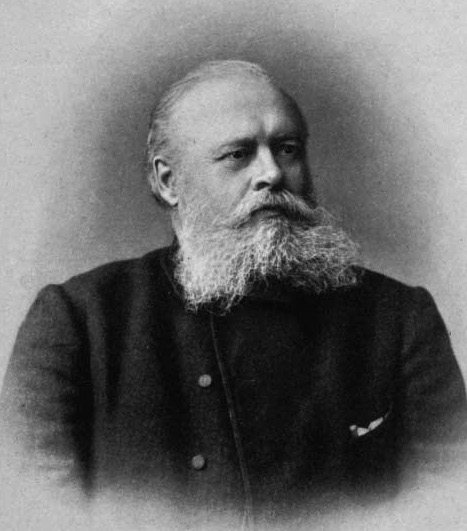
\includegraphics[width=\linewidth]{images/book2/markovnikov.jpg}
\end{minipage}\hfill
\begin{minipage}[t]{0.76\linewidth}\vspace{0pt}
व्लादिमीर मार्कोवनिकोव ने अपना नियम उन्नीसवीं शताब्दी में उन
उत्पादों से प्रतिपादित किया जो उन्होंने और अन्य लोगों ने प्रेक्षित किए थे, \omterm{def:b1:electronic-effects:intermediates}{कार्बधनायनों} या \omterm{def:b1:electronic-effects:curly-arrow}{वक्र तीरों} के
अस्तित्व से बहुत पहले: प्रकृति की एक नियमितता, जो अपनी व्याख्या संभव होने से पहले
लिख दी गई। \omterm{def:b1:electronic-effects:intermediates}{कार्बधनायन} स्थायित्व के माध्यम से उसका आधुनिक कथन दिखाता है कि
क्रियाविधि किसी आनुभविक नियम में क्या जोड़ती है: वह बताती है कि नियम कब विफल होना चाहिए।
(1905 में प्रकाशित एक शोक-सूचना से लिया गया चित्र, सार्वजनिक अधिकार-क्षेत्र,
विकिमीडिया कॉमन्स।)
\end{minipage}
\end{history}

\section{अभ्यास}

\begin{exercise}[$\star$]\label{exo:b1:electrophilic-additions:1}
इनका मुख्य उत्पाद बताइए: प्रोपीन + HCl; 2-मेथिलप्रोपीन + HBr;
1-मेथिलसाइक्लोहेक्सीन + HBr; ब्यूट-2-आइन + HCl का एक तुल्यांक।
\end{exercise}

\begin{exercise}[$\star$]\label{exo:b1:electrophilic-additions:2}
एथीन, साइक्लोहेक्सीन और प्रोपीन के साथ ब्रोमीन के उत्पाद लिखिए। उनके नाम
बताइए।
\end{exercise}

\begin{exercise}[$\star$]\label{exo:b1:electrophilic-additions:3}
हर ऐल्कीन का अम्ल-उत्प्रेरित \omterm{def:b1:electrophilic-additions:hydration}{जलयोजन} कौन-सा ऐल्कोहॉल देता है:
प्रोपीन, 2-मेथिलप्रोपीन, मेथिलीनसाइक्लोहेक्सेन?
\end{exercise}

\begin{exercise}[$\star$]\label{exo:b1:electrophilic-additions:4}
इनमें से कौन-से यौगिक सोडियम ऐमाइड से अभिक्रिया करते हैं: प्रोपाइन, ब्यूट-2-आइन,
प्रोपीन, एथेनॉल? अभिक्रियाएँ लिखिए।
\end{exercise}

\begin{exercise}[$\star\star$]\label{exo:b1:electrophilic-additions:5}
2-मेथिलप्रोपीन के \omterm{def:b1:electrophilic-additions:hydration}{जलयोजन} की पूरी क्रियाविधि \omterm{def:b1:electronic-effects:curly-arrow}{वक्र
तीरों} के साथ लिखिए, और समझाइए कि गरम सांद्र अम्ल में उत्क्रम अभिक्रिया को
वरीयता क्यों मिलती है।
\end{exercise}

\begin{exercise}[$\star\star$]\label{exo:b1:electrophilic-additions:6}
हैमंड अभिगृहीत से समझाइए कि 2-मेथिलप्रोपीन HCl से प्रोपीन की तुलना में
कहीं अधिक तेज़ी से अभिक्रिया क्यों करती है।
\end{exercise}

\begin{exercise}[$\star\star$]\label{exo:b1:electrophilic-additions:7}
ब्रोमीन साइक्लोहेक्सीन से अभिक्रिया करती है। दिखाइए कि उत्पाद
\textit{trans}-1,2-डाइब्रोमोसाइक्लोहेक्सेन है, और बताइए कि क्या वह \omterm{def:b1:stereochemistry-in-depth:stereocentre}{किरैल} है और
क्या उत्पाद प्रकाशतः सक्रिय है।
\end{exercise}

\begin{exercise}[$\star\star$]\label{exo:b1:electrophilic-additions:8}
3-मेथिलब्यूट-1-ईन पर HCl के उस योग की क्रियाविधि प्रस्तावित कीजिए जो
मुख्यतः 2-क्लोरो-2-मेथिलब्यूटेन देता है।
\end{exercise}

\begin{exercise}[$\star\star$]\label{exo:b1:electrophilic-additions:9}
प्रोपाइन और एक हैलोऐल्केन से हेक्स-2-आइन का, और
प्रोपाइन और बेंज़ैल्डिहाइड से 1-फ़ेनिलब्यूट-2-आइन-1-ऑल का एक संश्लेषण प्रस्तावित कीजिए।
\end{exercise}

\begin{exercise}[$\star\star\star$]\label{exo:b1:electrophilic-additions:10}
दोनों ब्यूट-2-ईनों पर ब्रोमीन के योग के त्रिविम रसायन को
चित्र द्वारा सिद्ध कीजिए: ब्रोमोनियम आयन, हर कार्बन पर प्रति आक्रमण, उत्पादों का \omterm{def:b1:stereochemistry-in-depth:representations}{क्रैम निरूपण},
वर्णक। हर स्थिति में बनने वाले \omterm{def:b1:stereochemistry-in-depth:isomers}{त्रिविम समावयवी}
गिनिए।
\end{exercise}

\begin{exercise}[$\star\star\star$]\label{exo:b1:electrophilic-additions:11}
प्रोपीन के साथ ब्रोमीन जल मुख्य उत्पाद के रूप में 1-ब्रोमोप्रोपेन-2-ऑल देता है।
स्थान-रसायन की व्याख्या कीजिए: जल ब्रोमोनियम आयन के अधिक प्रतिस्थापित
कार्बन पर आक्रमण क्यों करता है?
\end{exercise}

\begin{exercise}[$\star\star\star$]\label{exo:b1:electrophilic-additions:12}
एक हाइड्रोकार्बन \ce{C5H10} ब्रोमीन जल को रंगहीन कर देता है और HBr जोड़कर
2-ब्रोमो-2-मेथिलब्यूटेन देता है; उसका \omterm{def:b1:electrophilic-additions:hydration}{जलयोजन} 2-मेथिलब्यूटेन-2-ऑल देता है। दो
संभावित संरचनाएँ ज्ञात कीजिए और उन्हें अलग पहचानने का एक ढंग प्रस्तावित कीजिए।
\end{exercise}

\section{समस्या: दो ब्यूटीन और ब्रोमीन}

\begin{problem}[{सप्ताहांत समस्या --- दोनों ब्यूट-2-ईन, ब्रोमोनियम
क्रियाविधि, मेसो और रेसेमिक डाइब्रोमाइड, उनका प्रकाशिक घूर्णन और
प्राप्त द्रव्यमान}]
\label{pb:b1:electrophilic-additions:1}
एक प्रयोगशाला के पास ब्यूट-2-ईन की दो बोतलें हैं, एक शुद्ध \cip{Z}, एक शुद्ध
\cip{E}, और वह हर एक के \qty{5.60}{g} को डाइक्लोरोमेथेन में ब्रोमीन से
उपचारित करती है। मोलर द्रव्यमान (\unit{g/mol}): \ce{C4H8} 56.0, \ce{Br2}
159.8, \ce{C4H8Br2} 215.8।

\medskip
\noindent\textbf{भाग I --- दोनों ऐल्कीन।}
\begin{enumerate}
  \item \cip{Z}- और \cip{E}-ब्यूट-2-ईन खींचिए और वर्णकों का औचित्य दीजिए।
  \item क्या वे \omterm{def:b1:stereochemistry-in-depth:isomers}{त्रिविम समावयवी} हैं? \omterm{def:b1:stereochemistry-in-depth:enantiomers}{प्रतिबिंबरूपी} या \omterm{def:b1:stereochemistry-in-depth:enantiomers}{अप्रतिबिंबरूपी}?
  \item वे कमरे के ताप पर एक-दूसरे में क्यों नहीं बदलतीं?
  \item कौन-सी अधिक स्थायी है, और क्यों?
  \item ब्रोमीन के योग का समग्र समीकरण लिखिए।
  \item 2,3-डाइब्रोमोब्यूटेन में कितने त्रिविम केंद्र हैं? अधिक से अधिक कितने
        \omterm{def:b1:stereochemistry-in-depth:isomers}{त्रिविम समावयवी}, और वास्तव में कितने?
\end{enumerate}

\medskip
\noindent\textbf{भाग II --- क्रियाविधि।}
\begin{enumerate}[resume]
  \item \omterm{def:b1:electronic-effects:curly-arrow}{वक्र तीरों} के साथ ब्रोमोनियम आयन का बनना लिखिए।
  \item खुले \omterm{def:b1:electronic-effects:intermediates}{कार्बधनायन} के बजाय सेतुबद्ध ब्रोमोनियम आयन क्यों बनता
        है?
  \item ब्रोमाइड द्वारा आयन का खुलना लिखिए।
  \item ब्रोमाइड सेतु के विपरीत फलक से आक्रमण क्यों करता है?
  \item परिणामस्वरूप किस प्रकार का योग होता है?
  \item विलायक डाइक्लोरोमेथेन क्यों है, जल क्यों नहीं?
\end{enumerate}

\medskip
\noindent\textbf{भाग III --- उत्पाद।}
\begin{enumerate}[resume]
  \item \cip{E}-ब्यूट-2-ईन से: C2 पर आक्रमण का उत्पाद खींचिए और
        C2 तथा C3 के वर्णक बताइए।
  \item C3 पर आक्रमण के लिए भी यही। तुलना कीजिए।
  \item दिखाइए कि उत्पाद मेसो है।
  \item \cip{Z}-ब्यूट-2-ईन से: दोनों उत्पाद और उनके
        वर्णक खींचिए।
  \item वे किन अनुपातों में बनते हैं? मिश्रण का नाम बताइए।
  \item क्या अभिक्रिया त्रिविमविशिष्ट है? औचित्य दीजिए।
\end{enumerate}

\medskip
\noindent\textbf{भाग IV --- घूर्णन और द्रव्यमान।}
\begin{enumerate}[resume]
  \item \cip{Z} ऐल्कीन का उत्पाद कौन-सा प्रकाशिक घूर्णन दर्शाता है?
  \item हर ऐल्कीन की मात्रा परिकलित कीजिए।
  \item \qty{85}{\percent} \omterm{def:b1:extent-q-and-k:fractional-extent}{लब्धि} पर हर एक से अपेक्षित डाइब्रोमाइड का द्रव्यमान
        परिकलित कीजिए।
  \item \cip{E}-ब्यूट-2-ईन से प्राप्त डाइब्रोमाइड का \omterm{def:b1:stereochemistry-in-depth:optical-activity}{विशिष्ट घूर्णन}, और
        उसका प्राप्त द्रव्यमान, बताइए।
\end{enumerate}
\end{problem}
